%
% Extension
% Abschlussarbeit (Bachelor)
%
% Thema: Erstellung einer Browser Extension zur Usability Evaluierung von beliebigen Web-Applikationen über Heatmaps.
% Betreuer 1: Prof. Dr. Targo Pavlista
% Betreuer 2: Siamak Haschemi
%
% @author Christian Bromann <contact@christian-bromann.com>
%

\newglossaryentry{MHTML}{name=MHTML, description={MIME Encapsulation of Aggregate HTML Documents - ist die Zusammensetzung einer HTML Seite mit all ihren Ressourcen (referenzierte Skripte werden eingefügt und Bilder als base64 String umgewandelt)}}

\section{Extension}

Für die Durchführung der Tests und der Aufzeichnung der Daten ist die Chrome Extension verantwortlich. Sie muss bei jedem Probanden installiert sein, um am Test teilzunehmen. Dies ist sicherlich zu erst einmal hinderlich, da zum Einen nicht zu erwarten ist, dass ein Testuser diese Extension nutzen möchte, und zum Anderen, dass dieser auch einen Chrome Browser bei sich auf dem System installiert hat. Dennoch ermöglicht es den Nutzern von \textit{thEvaluator}, Testcases für jede beliebige Webseite zu erstellen und aus den Nutzerverhalten dieser zu lernen. Es ist ein Alleinstellungsmerkmal, welches am Ende Vorteile gegenüber Konkurrenzprodukten bringen kann.\\
\\
Da sich die Extension zum Zeitpunkt der Abgabe dieser Arbeit immer noch in einer Art Beta-Phase befindet, wird auf die Einbindung in den Google Web Store\footnote{\url{https://chrome.google.com/webstore}} verzichtet. Für den Beta-Test konnten sich die Probanden die Extension auf der offiziellen Projektwebsite\footnote{\url{http://qcentral.org/}} herunterladen. Da Google es verbietet fremde Extension mit einem einfachen Klick in den Browser einzubinden, muss diese erst heruntergeladen werden und via Drag\&Drop auf die Extensionseite\footnote{\url{chrome://extensions/}} des Browsers gezogen werden. Erst dann wird die Installation von Store-fremden Extensions gestattet. Ist dies erledigt erscheint in der Extension-Bar des Chrome Browsers ein kleines buntes Icon der \textit{thEvaluator}-Erweiterung. Klickt man darauf, so öffnet sich diese in einem kleinen Fenster. Zu sehen ist eine kleine Erläuterung zum Vorgehen des Tests und eine Textbox, in der die Testcase-ID eingegeben werden muss.

\begin{center}
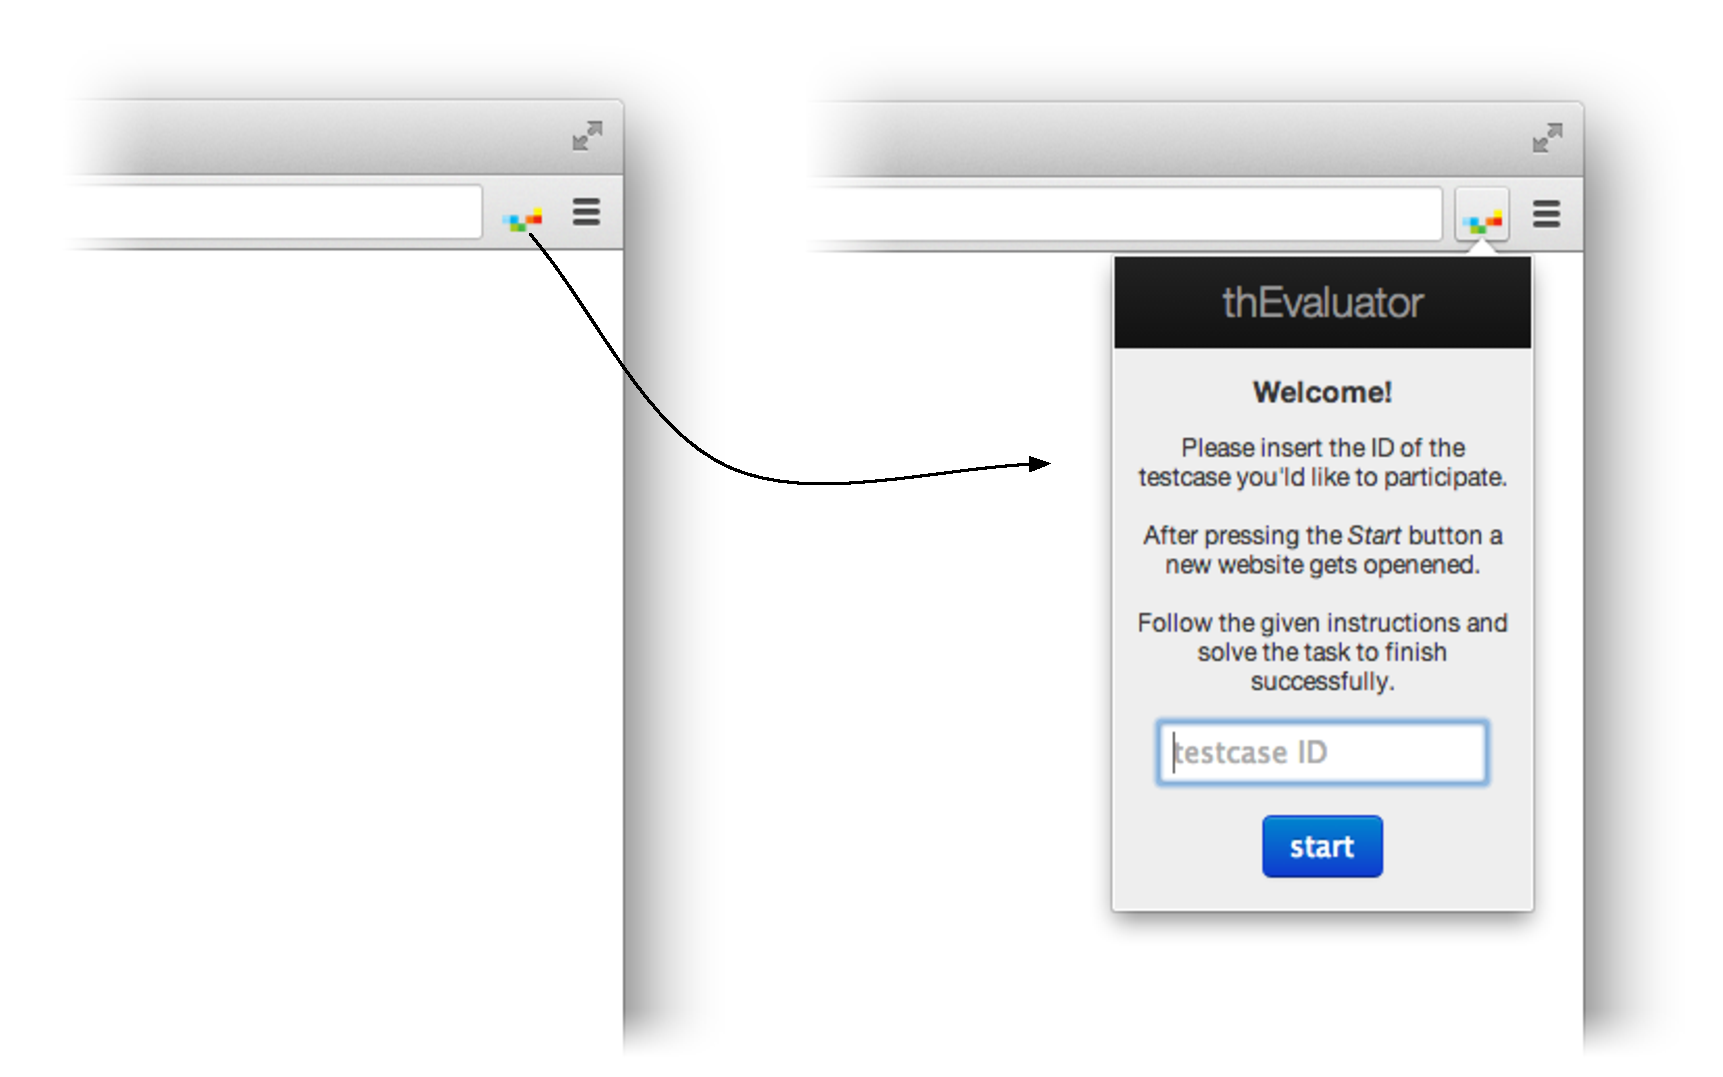
\includegraphics[scale=0.55]{./images/extension}
\end{center}
\begin{figure}[htb]
   \centering
   \caption{Aussehen der \textit{thEvaluator} Extension im Chrome Browser\\nach der Installation}
    \label{extension}
\end{figure}

Sobald der Proband die 10-stellige ID eingegeben hat und den \textit{start} Button drückt, beginnt der Testlauf. Die Extension öffnet dann einen neuen Tab und leitet den User auf die Start-URL.

\subsection{Aufbau}

Die Inhaltsstoffe einer Chrome Extension sind ganz normale HTML, CSS und JavaScript Dateien. Zusammengehalten wird alles durch ein Manifest, welches die Inhaltsstoffe auflistet und Rechte und Restriktionen festlegt. Jeder Nutzer bekommt bei der Installation angezeigt, welche diese sind und kann entscheiden, ob er sie zulassen möchte.
\\
\begin{lstlisting}[caption=Auszug aus der Manifest.json der \textit{thEvaluator} Extension,label=manifest]
{
    "manifest_version": 2,
    "name": "thEvaluator",
    "version": "0.1",
    "description": "Chrome extension to start thEvaluator usability tests",
    "browser_action":   {
        "default_icon": "img/icon128.png",
        "default_popup": "index.html"
    },
    "icons": { 
        "16": "img/icon16.png",
        "...": "..."
    },
    "background": {
        "page": "background.html"
    },
    "permissions": [ "cookies", "tabs", "http://*/*", "https://*/*" ],
    "content_scripts": [{
        "js": [
            "js/thEvaluatorWidget.js",
            "..."
        ],
        "css": ["dist/injected.css"],
        "all_frames": true
    }],
    "web_accessible_resources": [
        "templates/task.tpl",
        "..."
    ]
}
\end{lstlisting}

Listing \ref{manifest} zeigt einen Auszug des Manifestes der \textit{thEvaluator} Chrome Extension. Neben Name, Versionsnummer und Beschreibung der Extension werden zusätzlich Icons bestimmt und die Rolle der einzelnen HTML Seiten festgelegt.\\
\\
Eine weitere Komponente der Extension sind die Grunt\footnote{\url{http://gruntjs.com/}} Tasks. Diese kümmern sich um das Testen und Kompilieren der Extension zu einem Paket und die anschließende Umwandlung zu einer Chrome Extension Datei mit der Endung \textit{.crx}. Grunt ist ein Task-Manager, basierend auf NodeJS, welcher durch Plugins erweitert werden kann und die Entwicklung von Web-Applikationen jeglicher Art automatisiert. Die Tasks werden dabei in einer zentralen Datei, dem Gruntfile, definiert und können jeder Zeit über die Konsole ausgeführt werden. Durch die Kompilierung der Extension durch Grunt werden die CSS und JavaScript Dateien zusammengefügt und minifiziert. Dadurch schrumpft die Dateigröße der Erweiterung und macht den Sourcecode unlesbar.


\subsection{Architektur}

Eine Chrome Erweiterung besteht meist aus drei Komponenten. Einer \textbf{{\color{red}Background Page}}, die im Hintergrund des Browsers ausgeführt wird und die Hauptlogik enthält, einer Seite für die \textbf{{\color{green}Extension UI}}, die für die Ansicht und Logik des Extension-Fensters (PopUp) zuständig ist, und zu guter letzt einem \textbf{{\color{blue}Contentscript}}, die mit der angezeigten Seite des Browser interagieren kann \cite{extensionArchitecture}.

\begin{center}
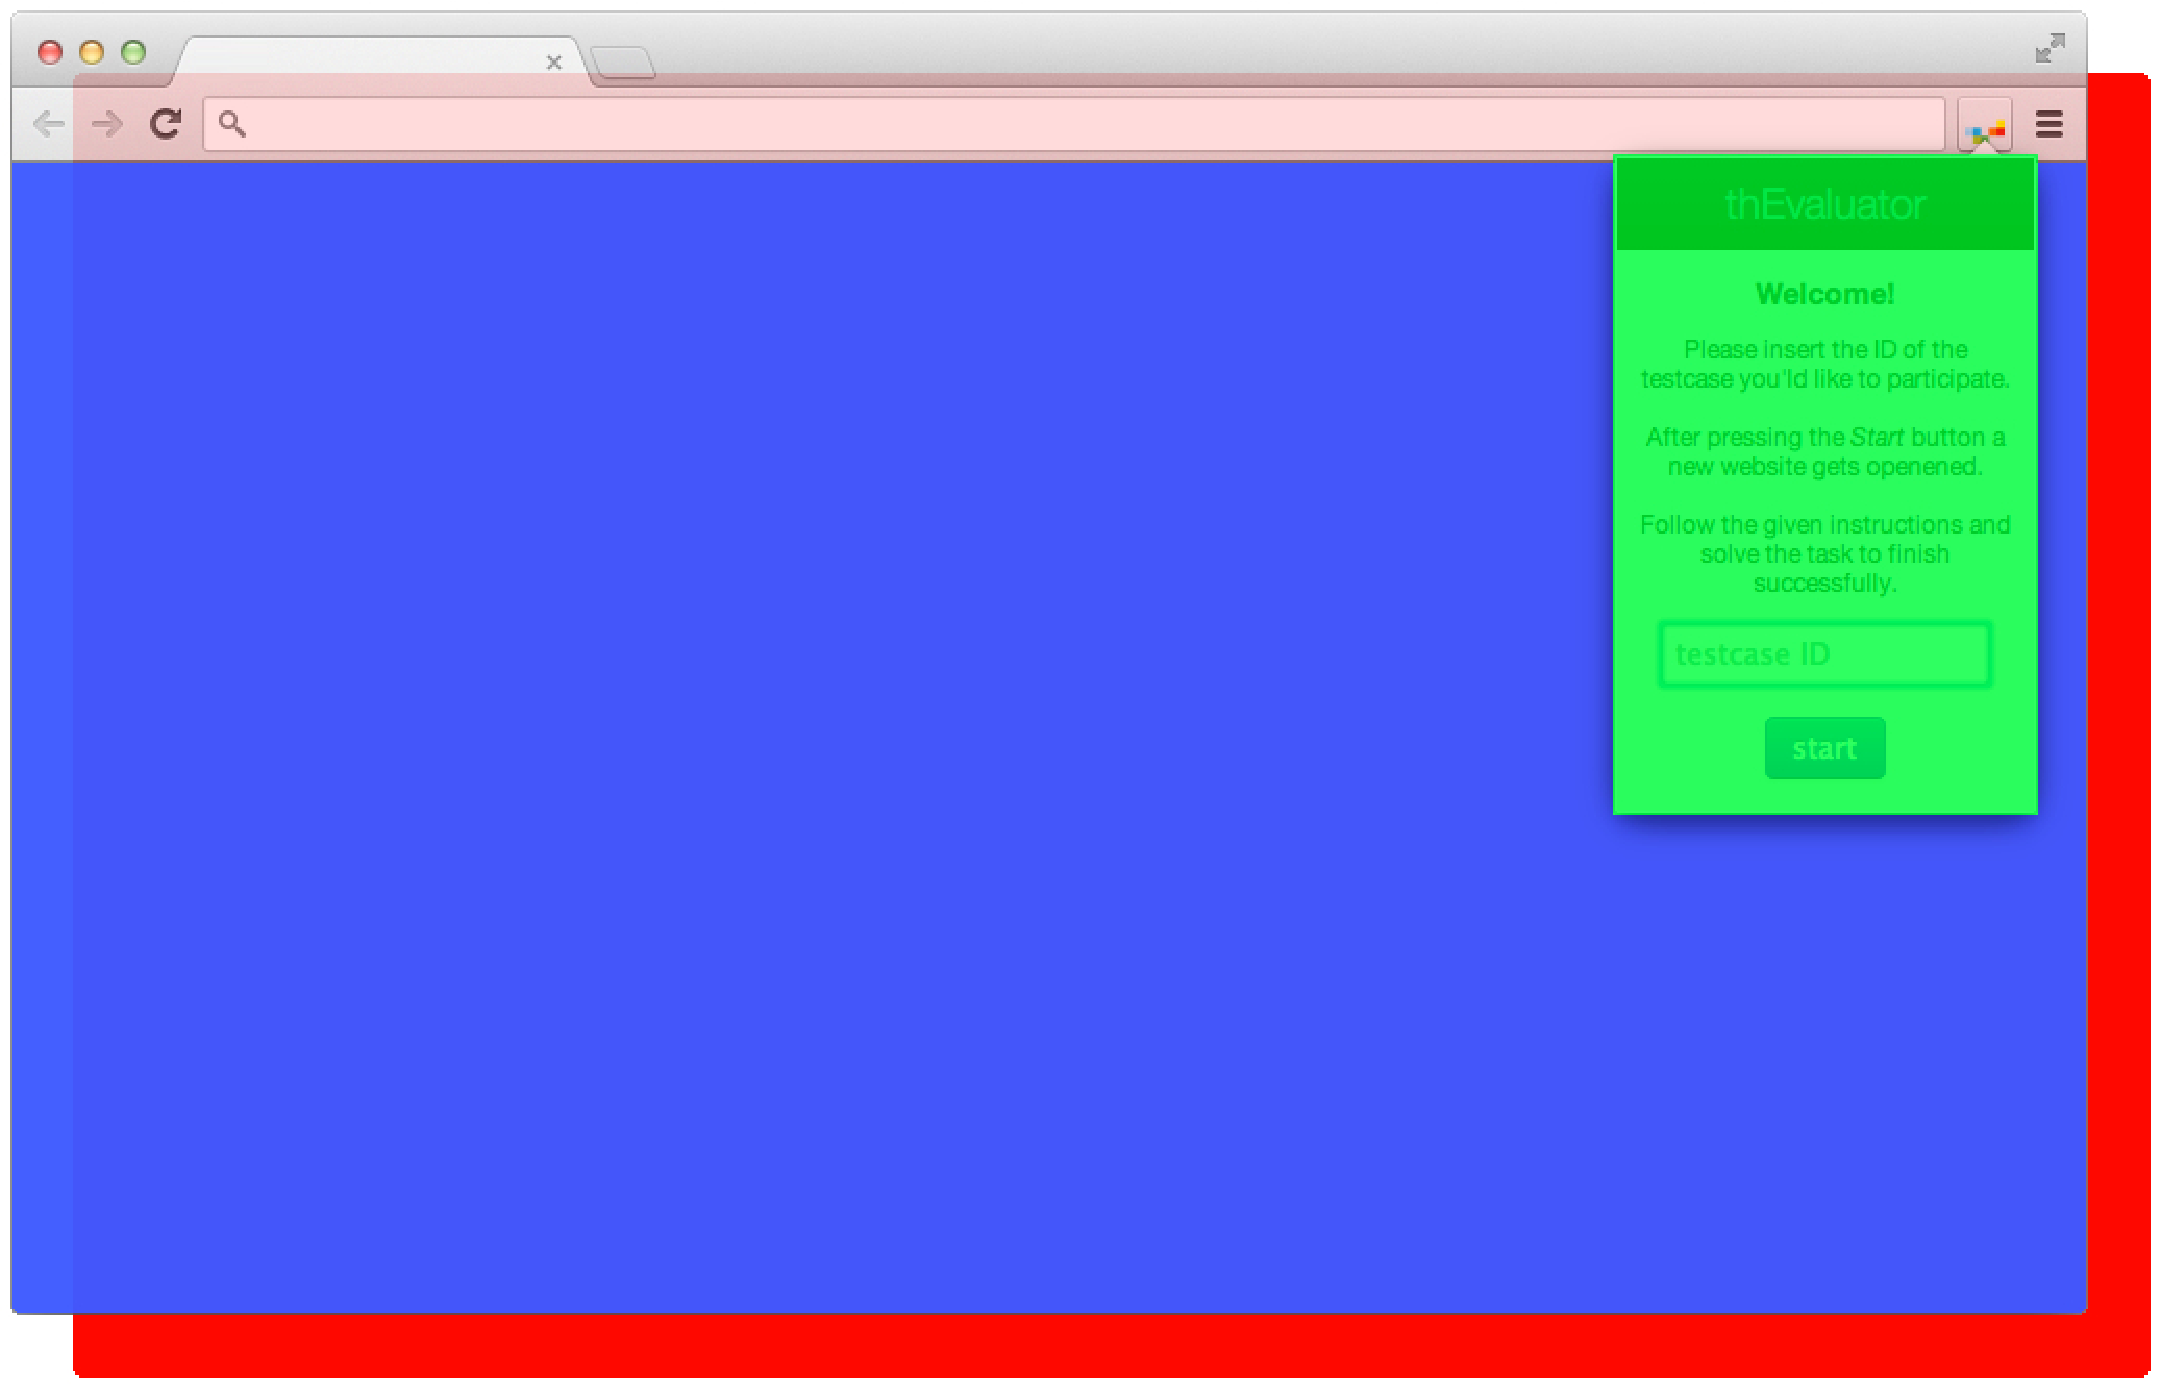
\includegraphics[scale=0.35]{./images/layers}
\end{center}
\begin{figure}[htb]
   \centering
   \caption{Die 3 Komponenten einer Chrome Extension}
    \label{layers}
\end{figure}

Die Laufzeiten der jeweiligen Komponenten sind sehr unterschiedlich. Während die Background Page und dessen JavaScripte dauerhaft ausgeführt werden, passiert dies für den UI Teil erst wenn das PopUp, durch den Klick auf das Extension Icon, geöffnet wird und auch nur die Zeit, solange es geöffnet ist. Das Contentscript dagegen wird immer dann vom Browser ausgeführt, sobald eine neue Seite geladen wird. Es verhält sich somit wie ein Script, welches in jeder Seite eingebunden ist. Es hat es Zugriff auf den DOM der Seite, somit auch auf dessen Struktur, und den Umgebungs- und globalen Variablen.\\
\\
In der \textit{thEvaluator} Extension findet die meiste Aktivität im Contentscript statt. Da die Erweiterung ständig die Mausposition abfragen muss, benötigt es Zugriff auf die globale \textit{window} Variable der Seite. Zudem werden Templates in den DOM gehangen, um eine neue Aufgabe anzuzeigen oder dem User die Information zu geben, welche er gerade bearbeitet. Die UI Page ist dafür verantwortlich die ID des Testcases aufzunehmen und sie anschließend der Background Page zu senden. Konnte die ID erfolgreich identifiziert und zugeordnet werden, wechselt das User Interface und die Aufgabenstellung wird angezeigt. Zusätzlich bietet ein \textit{Stop} Button die Möglichkeit den Testlauf zu beenden. Sobald die Background Page von dem PopUp die ID des Testcases bekommen hat, startet sie eine Socket Verbindung mit dem Server und erhält die Daten des Testcases, sowie dessen Aufgaben. Es öffnet die Start-URL in einem neuen Tab und sendet dem Contentscript eine Nachricht mit den Daten des Testcases. Dieses beginnt nun mit der ersten Frage. Da es nach jedem Seitenaufruf neu initialisiert wird, speichert es seine Umgebungsvariablen, wie zbs. die aktuelle Aufgabennummer, als Cookie ab.


\subsection{Nachrichtenübermittlung}

Die Komponenten der Chrome Extension müssen häufig miteinander kommunizieren. Die Background Page sendet z.B. bei jedem neuen Seitenaufruf die Daten des aktuellen Testcases und initialisiert damit das Contentscript. Dieses sendet jegliche Mauspositionen an die Background Page, damit sie diese via Socket Stream an den Server weiterleiten kann. Die Kommunikation findet dabei über das Message Passing statt \cite{messagePassing}. Jede Komponente kann auf Nachrichten reagieren oder sie selber senden. Dabei ist es sogar möglich Nachrichten an eine andere Extension zu senden, solange dessen ID bekannt ist. Es gibt dabei zwei Arten der Übertragung. Langzeitverbindungen halten einen dauerhaften Kontakt zwischen zwei Komponenten einer Extension. Typischer Use-Case wäre eine Autoformfill-Extension, die bei jeder Eingabe eines Buchstaben im Formular eine Möglichkeit zur Füllung des Formulars anbietet. Die \textit{thEvaluator} Extension nutzt ausschließlich sogenannte \textit{One-Time Requests}. Dabei handelt sich, um einfache Request mit einer JSON Nachricht. Diese besitzen jeweils ein \textit{action} Attribute, die für eine bestimmte Funktion im Contentscript bestimmt ist. Listing \ref{message} zeigt, wie jede Nachricht an eine Funktion im Contentscript zugewiesen wird. Das Objekt, welches diese Funktionen bereitstellt, nennt sich \textit{thEvaluatorInjected} und beinhaltet die Hauptlogik des Contentscripts. Da im Backgroundscript aus Einfachheitsgründen die Funktionen global deklariert werden, regelt eine \textit{switch} Anweisung alle ankommenden Nachrichten.
\\
\begin{lstlisting}[caption=Message Handeling im Contentscript,label=message]
var thEvaluator = new thEvaluatorInjected();
chrome.extension.onMessage.addListener(function(request,sender,sendResponse){

    if(typeof thEvaluator[request.action] === 'function') {
        thEvaluator[request.action](request,sender,sendResponse);
    } else {
        thEvaluator.log('couldn\'t find action: \'' + request.action + '\'');
    }

});
\end{lstlisting}

\subsection{Screenshotaufzeichnung}

Hinter jedem Klick des Users steckt in den häufigsten Fällen ein visuelles Ziel. Ob Link oder Bild, Internetnutzer erkennen ziemlich schnell, wohin man klicken muss, um auf eine neue Seite zu gelangen. Beim durchforsten der Seite ist häufig zu beobachten, dass User die Maus benutzen, um Texte zu erfassen. Der Mauszeiger wird dabei wie eine Art Finger benutzt, der Wort für Wort das Lesen begleitet. Diese visuellen Hintergründe sind daher bei der Auswertung von Heat- oder Clickmaps unersetzlich und helfen die Gründe für das Verhalten des Benutzers herauszufinden. Es ist daher wichtig, das hinter den X und Y Daten ein Bild steckt, zu dem diese zugeordnet werden können.\\
\\
Das Aufnehmen eines Screenshots ist in Google Chrome schwerer als anfangs vermutet. Die API bietet zwar die Möglichkeit, den aktuell sichtbaren Bereich zu scannen, jedoch nicht die komplette Seite. Eine Ausweichmöglichkeit wäre die Erzeugung von \Gls{MHTML} Dateien. Diese würden eine 1 zu 1 Kopie der ursprünglichen Seite abbilden und könnten bei der Auswertung in iFrames angezeigt werden. Da jedoch jegliche Bilder und Skripte in die Datei einfließen, ist der Speicheraufwand zu groß und für das Abscannen vieler Seiten ungeeignet. Daher muss ein Algorithmus die API erweitern, um einen Screenshot der ganzen Seite zu erhalten.\\
\\
In einer Art rekursiven Funktion tastet sich der Algorithmus über die Seite und nimmt sie dabei Stück für Stück auf. Dies geschieht im Skript der Background Page, da lediglich diese die Rechte zur Nutzung der Funktion besitzt. Ist ein Bereich abgescannt, so erhält das Contentscript die Nachricht ein Stück weiter zu scrollen, um einen neuen Teil der Webseite abzuscannen. Ist die Seite abgescrollt ruft die Funktion einen Callback auf und springt damit aus ihrer Rekursivität. Listing \ref{captureVisibleTab} zeigt als erstes die Funktion, die den sichtbaren Teil des Bildschirms einscannt und das Bild in einem Canvas zwischenspeichert.
\\
\begin{lstlisting}[caption=Funktion zum Abscannen des aktuell sichtbaren Bereiches der Seite,label=captureVisibleTab]
capturePage = function(opt,cb) {

    var x = opt.x,
        y = opt.y;

    console.log('take screenshot on %d , %d',x,y);

    chrome.tabs.getSelected(null, function(tab) {
        chrome.tabs.sendMessage(tab.id, {action: 'scroll', pos: {x:x,y:y}}, function(pos) {
            window.setTimeout(function() {
                chrome.tabs.captureVisibleTab(null, {
                    format: 'jpeg',
                    quality: 10
                }, function(data) {

                    if (data) {
                        var image = new Image();
                        image.src = data;

                        image.onload = function() {
                            screenshot.ctx.drawImage(image, pos.scrollX, pos.scrollY);
                            cb();
                        };
                    }

                });
            },150);
        });
    });

};
\end{lstlisting}

Wie in Zeile 9 zu erkennen ist, wird zuerst eine Nachricht an das Contentscript geschickt, auf eine bestimmte X und Y Position der Seite zu scrollen. Erst danach wird die Funktion zum Aufnehmen des Screenshots in Zeile 11 aufgerufen. Wie Zeile 10 zeigt, geschieht dies durch das \textit{setTimeout} erst nach 150ms. Grund dafür ist die Latenz, die durch das Rendern des neuen Bereiches der Seite entsteht. Da das Scrollen sprunghaft geschieht, braucht der Browser eine kurze Zeit, um die Inhalte anzuzeigen. Beim normalen scrollen fällt dies dem menschlichen Auge nicht auf. Bei einem Test wird der User zwar für eine kurze Zeit irritiert, da er die Scrollbewegung mitbekommt. Da dies jedoch für jede URL nur einmal geschieht, sind davon nur sehr wenige Testuser betroffen. Zudem hat dies keinen direkten Einfluss auf das Nutzerverhalten des Benutzers.\\
\\
Gesteuert wird dies durch die rekursive Funktion, die sich erst beendet, wenn der unterste Bereich der Seite erreicht wurde. Die Rekursivität entsteht dadurch, dass der Callback der Funktion \textit{capturePage} die Funktion selber ist und aufgerufen wird, sobald der Screenshot genommen wurde.
\\
\begin{lstlisting}[caption=Rekursive Funktion die das Abscannen der Seite steuert,label=takeScreenshot]
takeScreenshot = function(opt,cb) {

    var x = opt.x || 0,
        y = opt.y || 0;

    if(y < docDimension.height) {
        capturePage({x:0,y:y}, function() {
            takeScreenshot({x:0, y: y + docDimension.innerHeight }, cb);
        });
    } else {
        cb();
    }
},
\end{lstlisting}
\vspace{0,5cm}

Aktuell wird lediglich die vertikal Achse abgescannt. Da die meisten Webseiten sich in der Vertikalen ausbreiten, reicht dies vorerst aus. Hier könnte jedoch der Algorithmus derart erweitert werden, dass die Funktion erst dann aus der Rekursivität springt, sobald auch die X Achse abgescrollt wurde.